% For easier proof-reading, use the single-column, double-spaced layout:
%\documentclass{IWORK2014}
% Final Paper use double-column, normal line spacing. Comment the
% above line and uncomment the following line when you are writing
% Full paper and Final paper!  
\documentclass[cameraready]{IWORK2014}

\usepackage[hyphenbreaks]{breakurl}
\usepackage{hyperref}
\usepackage{tabularx}
\usepackage{graphicx}

\begin{document}

%=========================================================

\title{Bio-Inspired Networking}

\author{Juha Viljanen\\
        Aalto University School of Science \\
	\texttt{juha.o.viljanen@aalto.fi}}
\maketitle

%==========================================================

\begin{abstract}
In nature evolution has made sure that only the fittest biological organisms and systems survive. They tend to have simple and elegant solutions to complex problems arising from challenging environmental conditions. Throughout history, man has drawn inspiration from nature's solutions to solve issues in totally different fields. In recent decades these nature and biology inspired approaches have been applied to the field of computer science and networking.

Developing bio-inspired solutions is typically divided into three steps: Finding the analogies between the contexts of a technical problem and the biological system; deepening the understanding on the biological system; simplifying the biological patterns and applying them to the technical solution.

This paper takes a closer look at two bio-inspired networking solutions: the A-ESR algorithm and the Physarum Optimization. A-ESR is drawn from higher level understanding of a biological system: a foraging ant colony. The algorithm is used in the Internet infrastructure to optimize its energy consumption. Physarum Optimization draws understanding from a lower abstraction level: the functions of a simple cellular organism. It is used to find the minimum exposure path of a wireless sensor network, i.e. finding the path between two predefined points in a sensor-covered area that has the least sensor-coverage.

This paper looks at similarities and differences between the two approaches and considers some other possible application areas for them.

\vspace{3mm}
\noindent KEYWORDS: bio-inspired, networking, Ant Colony Optimization, A-ESR, Physarum Optimization

\end{abstract}

%============================================================


\section{Introduction}

Nature provides different mechanisms to solve complex problems in pragmatic, efficient and elegant ways. There is a lot that we can learn from Nature and apply to the world of computing and networking. One can find analogies between the different players and functions of a specific system in nature and a technical problem, for example in the networking domain \cite{dressler2010bio}.

Inspiration has historically been drawn from a higher level understanding of biological systems in Nature \cite{kroeker2011biology}, \cite{liu2012physarum}. A representative example of this is the sophisticated way ants indirectly communicate with each other while foraging. They do not need any centralized controlling unit nor do they ever need to have physical contact with each other. By leaving and following the right pheromone trails specified by a certain set of rules, they are able to coordinate their foraging in an efficient and autonomous way. A similar solution has been adapted and applied to modern routing protocols \cite{dressler2010bio}.

Today, also solutions from low level biological systems, such as molecular systems \cite{kroeker2011biology} or simple cellular organisms \cite{liu2012physarum}, are adapted to the field of computer science. For example, the neurological development of fruit-flies has inspired a minimalistic and efficient algorithm for self-organizing distributed networks \cite{kroeker2011biology}.

Bio-inspired approaches are employed in three main areas, namely computing, systems and networking \cite{dressler2010bio}. In the area of computing, bio-inspired approaches are exploited to improve the efficiency of computation algorithms, for example in optimization processes or pattern matching. Regarding the systems area, research is ongoing to design system architectures of massivley distributed, collaborative systems, while the area of networking is already benefiting from efficient and scalable networking solutions and autonomous organizing in a distributed environment.

Bio-inspired approaches offer qualities attractive to the networking field. They offer feasible solutions for achieving the demanding characteristics of next generation network architectures. The most challenging characteristics are the dynamic nature of mobile and ad-hoc networks and cognitive radio networks, autonomous operation in a infrastructureless network and communication in nano and micro scale networks \cite{dressler2010bio}. In large, heterogenous networks, the most efficient solutions do not usually include a centralized controlling entity, but favor a self-organizing, learning and evolving type of agents traversing and finding optimal routes through the network \cite{dressler2010bio}.

Biological systems often have a small set of simple rules that can be used to create complex behavior \cite{dressler2010bio} for solving challenging problems. These solutions usually possess qualities such as self-organization \cite{kroeker2011biology}, adaptation to changing environmental conditions, fault tolerance, efficient management of scarce resources, collaboration and survival to harsh conditions \cite{dressler2010bio}.

Section 2 presents the background. Section 3 presents an Ant Colony Optimization algorithm called A-ESR. Section 4 presents the Physarum Optimization algorithm. In the conclusions the two algorithms are compared with each other and future aspects are presented.

\section{Background}

\begin{figure*}
    \centering
    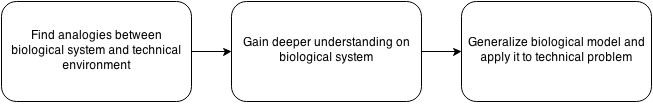
\includegraphics[width=0.8\textwidth]{bio-inspired-steps.png}
    \caption{Steps in developing a bio-inspired approach}
    \label{fig:bio-inspired-steps}
\end{figure*}

Developing a bio-inspired approach for issues in the engineering field is divided into three steps \cite{dressler2010bio} as shown in Figure \ref{fig:bio-inspired-steps}. At the beginning one needs to identify the analogies between the targeted technical environment and the biological system. How do the different players, structures and methods in the biological system correspond to those in the technical environment? Are there similarities? After finding the analogies, the next step is to research the biological system and try to understand it and its functions in a detailed and precise way. The third step is usually to generalize the biological model and to apply it to the chosen technical problem, hence to define the bio-inspired solution.

\begin{table*}
    \centering
	\begin{tabularx}{0.90\textwidth}{|X|X|X|X|}
		\hline \textbf{Biological principle} & \textbf{Description} & \textbf{General benefits} & \textbf{Applications in networking} \\ \hline
		Swarm intelligence & Behavior and interaction of large groups of insects, such as ants or bees & Autonomous route optimization & Routing, optimal node deployment, node localization, network clustering \\ \hline
		Firefly synchronization & Fireflies gather on trees and start to emit flashes in a synchronous manner. & Decentralized synchronization & Robust distributed clock synchronization, synchronized decentralized networks such as wireless ad hoc networks \\ \hline
		Artificial immune system & The natural immune system continuously scanning the body for pathogens and giving the proper resonse to them in non-specific or specific way depending on whether the specific pathogen is a known one or not & Detect and respond to intruders, self-learning and memorization & Misbehavior or intrusion detection, node and rate selection \\ \hline
		Cellular signalling pathways (Inter- and Intracellular communication) & Communication and interaction between and within cells of living organisms, such as the human body & Robustness, distributedness, efficiency, self-healing & Coordination and control in distributed systems, network clustering, protection \\ \hline
		DNA based & Approaches based on DNA and their subsegments such as Gene Regulatory Networks, their functions and interaction & Robustness and adaptation to the environment & Robust deployments of wireless sensor networks \\ \hline
	\end{tabularx}
	\caption{Categories of bio-inspired approaches in networking. Compiled based on \cite{hylsberg2011bioinspired, tyrrell2006fireflies, nazi2014deployment, zhang2013swarm}}
	\label{tbl:bio-categories}
\end{table*}

Bio-inspired networking can be divided into 5 categories based on their origins: swarm intelligence, firefly synchronization, artificial immune system, intercellular communication and DNA based approaches. Table \ref{tbl:bio-categories} decsribes them all briefly and gives examples of their application in networking. The category definitions of Hylsberg et al \cite{hylsberg2011bioinspired} was used as a basis for the table. DNA based approaches were added as the latest branch of bio-inspired networking. An example for an DNA based approach is the Gene Regulatory Networks based solution for robust sensor networks introduced by Nazi et al \cite{nazi2014deployment}. Additional information from \cite{tyrrell2006fireflies} and \cite{zhang2013swarm} were added to the classes used by Hylsberg et al.

This paper describes more closely two different bio-inspired approaches: Ant Colony Optimization and Physarum Optimization. Both are optimization algorithms based on the way biological entities or systems consisting of these are searching for food resources, i.e. are foraging. Ant Colony Optimization is a text book example of a bio-inspired approach based on a higher level understanding of a biological system: foraging ants. Physarum Optimization by contrast is based on a lower level understanding on how a slime mold, which is a simple cellular organism, works and how it behaviour has evolved \cite{liu2012physarum}.

\section{Ant Colony Optimization}
Ant Colony Optimization (ACO) is a form of bio-inspired solutions derived from the category of Swarm Intelligence \cite{hylsberg2011bioinspired}. One of its applications, the AntNet routing protocol, was introduced already in 1998 \cite{di1998antnet} with the purpose of exploiting ACO in order to improve the routing protocols efficiency in an autonomous fashion. More recently, Y.-M. Kim et al \cite{kim2012ant} proposed a new routing scheme called A-ESR to optimize network elements and hence to make the whole Internet more energy efficient, \cite{kim2011ant}. This section examines the A-ESR algorithm.

\paragraph{The technical problem and its context: Energy effient routing of Internet traffic}~\\
The infrastructure of the Internet is consuming more and more energy every year. In 2008, studies showed that the Internet consumed about 5.5\% of the world's total energy. This share was, at that time, expected to grow at a rate of 20-25\% annually \cite{proceedings2008energy}. A substantial portion of Internets power consumption could be reduced by optimizing the network elements, this making them more energy-efficient \cite{andrews2010routing}. Network elements use the same amount of power regardless of whether there is a lot of traffic going through them during peak hours, or whether they are in an idle state during low traffic hours \cite{gupta2007using}.

\paragraph{The biological system: Foraging ant colonies}~\\
Foraging ants of an ant colony are able to over time find the shortest paths from their nest to food sources in its environment \cite{dorigo1999ant, goss1989self}. They do this using indirect, local communication called stigmergy \cite{grasse1959reconstruction}. While moving between their nest and a food source the ants leave behind a chemical substance called pheromone \cite{ghosh2008aggregation}. A ant following a shorter path can complete it more frequently than one following a longer one. Hence the shorter paths get stronger pheromone trails. See Figure \ref{fig:aco} for a simplified case of the ant colonies route optimizing behavior.

\begin{figure*}
    \centering
    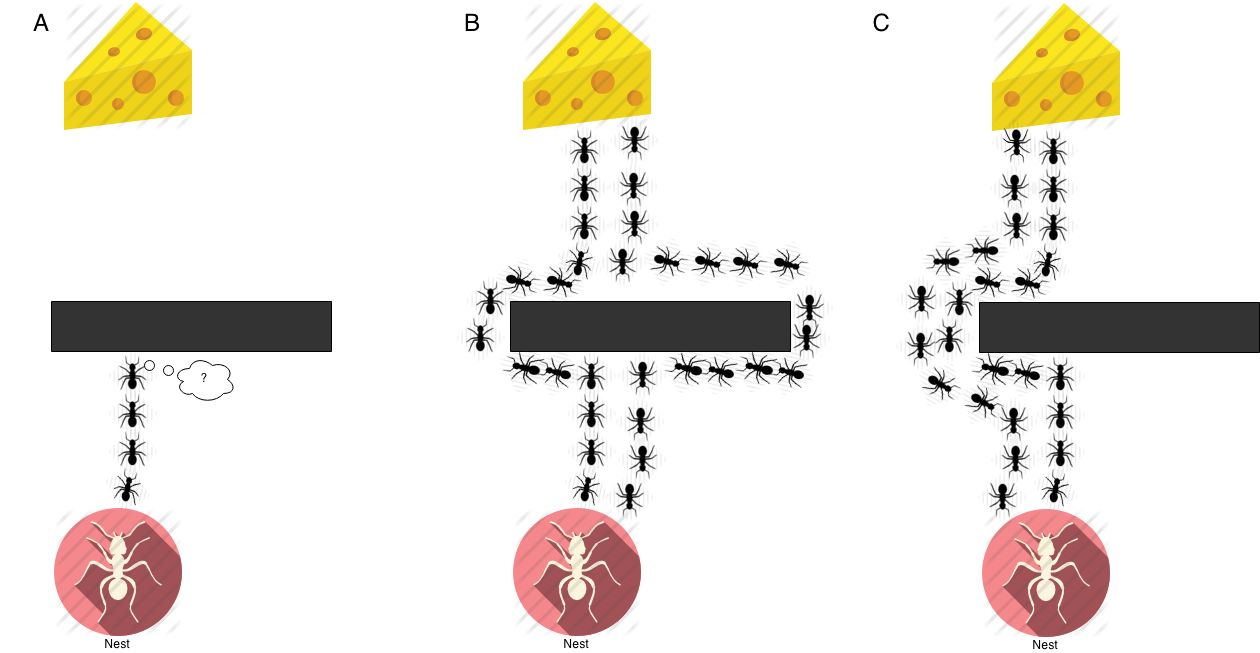
\includegraphics[width=0.8\textwidth]{aco.png}
    \caption{Foraging ant colony. A) An obstacle is between the nest and a food source. B) Ant find two routes that go around the obstacle. C) Ant are able to finish the shorter route quicker, thus making its pheromone trail stronger. It becomes the standard route to the food source.}
    \label{fig:aco}
\end{figure*} 

Ants prefer to move to a direction that has the most intense pheromone trace, which usually is the shortest path to a food source. This way the shortest paths quickly get significantly stronger pheromone trails and will attract even more ants. Over time the pheromone fades away. Hence longer routes or paths to food sources that have run out will completely fade away over time. A part of the ants does random searches to be able to find new food sources or new, shorter paths to old food sources \cite{dressler2010bio}.

\paragraph{Analogies and application: Basic concepts of ACO}~\\
The idea behind classic Ant Colony Optimization algorithm is to do path sampling in a network \cite{di2004ant, di2008theory}. The sampling is done traversing control data packets through the network and recording the performance and delays between each node. The control packages are generally referred to as agents or artificial ants. They will try out different paths between two arbitary points in the network. We distinguish between two types of agents: forward and backward ants.

Forward ants are created concurrently and independently at different nodes of the network. They have a predefined, but randomly chosen destination that they traverse to starting from the node they were created in. On their way to the destination they will follow a set of rules to find optimal routes. They gather information on all the delays between each jump between nodes.

Once a forward ant reaches its destination a backward ant is created to traverse the same way back to the origin of the forward node. On its way it will update the so called pheromone tables of each node. The pheromone tables are data structures that contain information on how good routes to different destinations traversing through its neighbour nodes are, i.e. the desirability of travesing to a node, $i$, next to the current node, $j$, when the packet destination is node $k$. The forward ants going through a node will choose the target of their next jump based on a stochastic rule that gives a higher probability to neighbour nodes that have stronger pheromone trails, i.e. are suggested by the pheromone table as an optimal path to the agents destination. The stochastic rule also applies a local heuristic function differing between ACO implentations. This way the exploration of new paths as well as load balancing of different routes can be accomplished.

\begin{table*}
    \centering
	\begin{tabularx}{0.90\textwidth}{|X|X|X|}
		\hline & \textbf{Foraging ant colony} & \textbf{Ant Colony Optimization} \\ \hline
		\textbf{Context} & Foraging ant colony & Networking \\ \hline
		\textbf{Problem} & Finding optimal paths to food sources & Finding optimal paths between network elements \\ \hline
		\textbf{Players} & Ants & Agents: forward and backward ants \\ \hline
		\textbf{Targets} & Food sources & Predefined destinations of each forward ant \\ \hline
		\textbf{Communication method} & Trails of chemical substance called pheromone & Numerical values written by backward ants to tables of each network element \\ \hline
	\end{tabularx}
	\caption{Analogies between foraging ant colonies and the Ant Colony Optimization algorithm}
	\label{tbl:analogies_ant}
\end{table*}

\paragraph{How the A-ESR algorithm differs from classic AOC}~\\
A-ESR stands for self-adaptive energy saving routing \cite{kim2012ant}. The main contribution of the A-ESR algorithm in comparison to other AOC algorithms is, that, in order to save energy of network elements, it shuts down links between nodes when their load is low. Traffic is aggregated to fewer more heavily loaded links. This way of aggregating traffic to the links that have the biggest load and shutting down the links that are now longer used for routing, is called traffic centrality. High traffic of links is communicated through pheromone trails in the pheromone tables of individual nodes. Table \ref{tbl:analogies_a-esr} sums up the novelties of the A-ESR algorithm.

\begin{table*}
    \centering
	\begin{tabularx}{0.90\textwidth}{|X|X|X|}
		\hline & \textbf{Foraging ant colony} & \textbf{A-ESR} \\ \hline	
		\textbf{Result} & Longer paths with weaker pheromone trails are become unused by ants. & Light loaded links with weak pheromone trails are shut down. \\ \hline
	\end{tabularx}
	\caption{More specific analogies between foraging ant colonies and the A-ESR algorithm (in addition to the ACO analogies).}
	\label{tbl:analogies_a-esr}
\end{table*}

\section{Physarum Optimization}
The Physarum Optimization approach exploits the cellular computation model of the slime mold physarum polycephalum in wireless sensor networks (WSN) \cite{liu2012physarum}. Out of the categories listed in Table \ref{tbl:bio-categories} Physarum Optimization fits best to the category of cellular signalling pathways, since it depends on communication between and within single physarum polycephalum cells. Physarum Optimization is used to solve the minimal exposure path problem of WSNs, which relateds to their worst case coverage. The approach is claimed to be simple and its processing highly concurrent. It should also be useful for designing new graph-algorithms, routing protocols and self-organizing network (SON) topologies.

\paragraph{The technical problem and its context: Wireless sensor networks}~\\
Wireless sensor networks consist of sensor nodes geographically distributed in an area \cite{nazi2013robust}. These sensor nodes collect data from their environment, process it by aggregating and filtering and forwarding it to other recievers in the sensor network. WSNs may be used in contexts of smart healthcare, disaster management, environment monitoring \cite{nazi2013robust} or even military applications \cite{liu2012physarum}.

WSNs can consist of sensors, let us say motion detectors, that aim to detect intruders coming to a restricted area. Generally the coverage of these areas is not complete and by an intruder might find uncovered paths through the restricted area, that would allow him to trespass without getting noticed. L. Liu et al \cite{liu2012physarum} aim to find the path, in such intruder detection scenario, which has the least sensor coverage and hence has the least risk of the intruder being detected by the sensors. This path represents the minimal exposure path. By identifying the minimal exposure paths one can find the weak spots of the covered area and add new sensors to that critical area, where they improve the areas coverage the most.

\paragraph{The biological system: Physarum Polycephalum}~\\
Physarum polycephalum is a large, single-celled amoeba-like organism which belongs to the family of slime molds \cite{liu2012physarum}. Its body has tube-like constructions that it uses to transfer nutrients, signals. Physarum moves by transporting body mass in these tubes. Physarum is known to avoid light. It has the ability to find optimal routes between food sources -- even if there were a maze separating them \cite{nakagaki2000intelligence}. In a dark, non-illuminated area the optimal route is the shortest route between the food sources. In an unevenly lit environment the optimal path is the one with the least risk of being exposed to light. As Figure \ref{fig:physarum} shows, physarum polycephalum can also be seen with the bare eye without using a microscope.

\begin{figure}
    \centering
    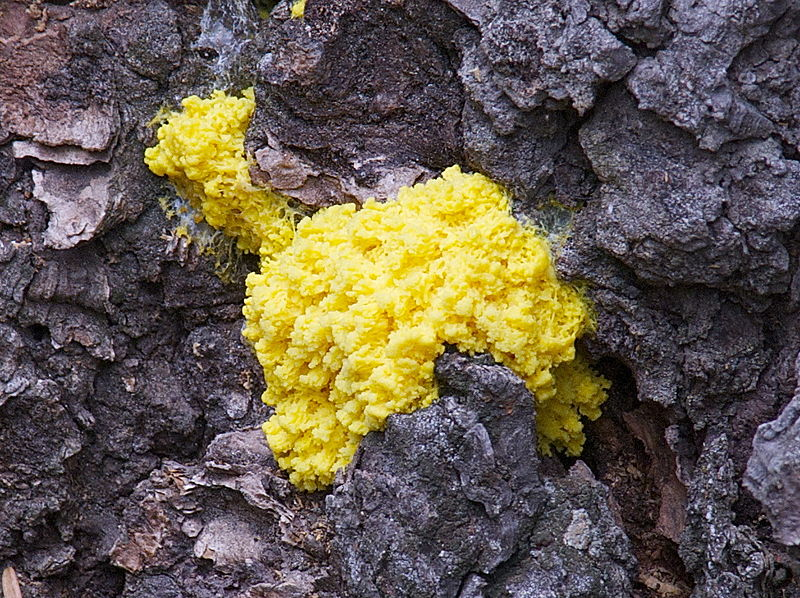
\includegraphics[width=0.8\linewidth]{physarum.jpg}
    \caption{Physarum plycephalum on the surface of a tree.
{\tiny Originally posted to Flickr as \href{http://flickr.com/photos/33466410@N00/4988821189}{Slime Mold (Physarium polycephalum)} by \href{http://flickr.com/people/33466410@N00}{Jerry Kirkhart}. The image is licenced under the \href{http://creativecommons.org/licenses/by/2.0/deed.en}{Creative Commons Attribution 2.0 Generic} license.}}
    \label{fig:physarum}
\end{figure}

Physarum polycephalum exists as a single-celled organism for as long as it has enough food sources available. When food sources are scarce, they start signaling each other to join and form a group. As a group they are able to function as a single body, or more precisely: a multicellular mass. In this state they are more sensitive to airbourne chemicals and can hence find food sources better. Frederick Spiegel, a biology professor at the University of Arkansas and an expert on slime molds describes a moving group of physarum looking like a "moving sausage" \cite{spiegel2012slimemold}.

\paragraph{Analogies and application: The Physarum Optimization algorithm}~\\
The analogy between Physarum finding the shortest path between food sources in an inhomogenously illuminated field and the trying to find the path having the worst sensor coverage in a wireless sensor network is simple. In the biological system the desired result is that Physarum does not catch light on his way to the food source. In the wireless sensor networks this corresponds to an intruder that does not want to be exposed to sensors while traversing between the selected target points in a sensor-covered area \cite{liu2012physarum}. Using these analogies the minimal exposure path problem of the WSNs can be solved using observations from Physarum's behaviour.

\begin{table*}
    \centering
	\begin{tabularx}{0.90\textwidth}{|X|X|X|}
		\hline & \textbf{Foraging Physarum Polycephalum} & \textbf{Physarum Optimization} \\ \hline
		\textbf{Context} & Foraging slime mold & Wireless Sensor Networks \\ \hline
		\textbf{Problem} & Finding optimal paths to food sources & Finding optimal paths between to predefined points \\ \hline
		\textbf{What defines an optimal path} & A path that has the least amount of light & A path with the least sensor coverage \\ \hline
		\textbf{Players} & Physarum & Intruder \\ \hline
		\textbf{Targets} & Food sources & Predefined destinations \\ \hline
	\end{tabularx}
	\caption{Analogies between foraging Physarum Polycephalum and the Physarum Optimization algorithm}
	\label{tbl:analogies_physarum}
\end{table*}

\section{Conclusion}

\paragraph{Comparison between ACO and PO}~\\
As Table \ref{tbl:aco-po-comparison} illustrates, the main benefits of both A-ESR and Physarum Optimization are their autonomous ways of working, which enforces local calculation and direct communication. No global state has to be maintained for a central controlling unit, which allows easy parallellization of the performed activities.

\begin{table*}
    \centering
	\begin{tabularx}{0.90\textwidth}{|X|X|X|}
		\hline & \textbf{Ant Colony Optimization, A-ESR} & \textbf{Physarum Optimization} \\ \hline
		\textbf{View point on biological system} & High level & Low level \\ \hline
		\textbf{Application field} & Computer networking; Energy efficient routing & Wireless Sensor Networks; Minimal sensor exposure path for sensors covered areas \\ 	\hline
		\textbf{Control system} & Locality (no central control necessary); Allows easy parallelity & Locality (no central control necessary); Allows easy parallelity \\ \hline
		\textbf{Aim and Result} & In order to save energy \textit{reduce} amount of active links between nodes & In order to improve sensor coverage find its weak spots so that sensor amount can be \textit{increased} in this area \\ \hline
	\end{tabularx}
	\caption{Comparison of the A-ESR and Physarum Optimization algorithms}
	\label{tbl:aco-po-comparison}
\end{table*}

A notable difference between the two algorithms are that their aims are exactly opposite to each other. The aim of A-ESR is to reduce the amount of active links in an network and hence to save energy. Physarum Optimization in turn aims to find the weak spots in the sensor coverage of a wireless sensor network so that the amount of sensors can be increased in those. Hence the sensor coverage can be improved.

\paragraph{Is there a general difference between high and low level inspired approaches?}~\\
The comparison between Physarum Optimization and A-ESR indicate that there is no substancial difference between bio-inspired approaches that are inspired by higher or lower level understanding of biolocial systems. They both follow the same rules for defining a bio-inspired solution that were defined by Dressler et al \cite{dressler2010bio}. What is more important is finding the analogies between the biological system and the technical environment. Hence the defining factor of bio-inspired solutions is not the abstraction level of their origin, but rather the type problems they are able to solve.

For example Hylsberg et al \cite{hylsberg2011bioinspired} list problem types and contexts that different biological systems are able to solve and have been successfully applied to. Swarm intelligence has, for instance, been applied to routing in computer networks, optimal node deployment, node localization, and network clustering, whereas the artificial immune system has been applied to misbehavior detection and intrusion detection systems.

\paragraph{Future aspects}~\\
As the A-ESR algorithm is used to save energy consumption of network elements routing Internet traffic, it might be worth investigating whether it would be as useful in the field of wireless sensor networks as well. One of the most important limiting factors in WSN is the limited available energy, which sets its challenges to the design of the used routing protocols \cite{hylsberg2011bioinspired}.

Many applications using Ant Colony Optimization in WSNs have been proposed \cite{bennis2013enhanced, zhang2004improvements, camilo2006energy, cai2006aco, sun2008asar, kiri2007self, ghasemaghaei2007ant}. These approaches have different goals ranging from fault tolerance \cite{zhang2004improvements} to reliability and scalability \cite{kiri2007self}. Many of the ACO based algorithms applied to WSN are energy aware \cite{saleem2011swarm}. Also completly othe solutions not applying bio-inspired approaches have been researched for energy effieciency in the WSN field \cite{wightman2008a3}. It would be interesting to see whether the A-ESR approach would be applicable in there and how it would perform in comparison to the other enegry efficient solutions.

In \cite{liu2012physarum} the context of use for Physarum Optimization is finding minimal sensor exposure paths in an area covered with sensors for example in the case of intruder detection with motion detectors. The authors indicate that the algorithm may also be applied to finding the shortest path in any kind of large scale graphs or inhomogeneous fields. An obvious place to try the algorithms performance would be to find minimal exposure paths of network coverage in WSNs or mobile networks. Once these are found one could improve the network coverage by adding new network elements to cover the area of the minimal exposure path.

%============================================================

\bibliography{references}
\end{document}

